\newpage\null\thispagestyle{empty}\newpage
\clearpage{\thispagestyle{empty}\cleardoublepage}
\part{Software implementation}
% \acbarrier
\parttoc
% 
% 
% 
\setcounter{chapter}{4}
\chapter{Dense nerve fiber modelling}
\label{chap:sof:modelling}
% 
In \cref{chap:neuro} the structure of nerve fibers and the macroscopic structure of \ac{WM} were described.
The question is how to represent such a structure in a computer algorithm?
For simple fiber configurations, \eg{} parallel, linear nerve fibers, this is relatively straightforward.
However, it has been shown that irregular, non-symmetric nerve fiber configurations are necessary to obtain a realistic result for microscopy simulations based on the wave nature of the light \cite{MenzelDissertation}.
Therefore, one needs ideally a representation, which allows building any kind of pattern.
\par
%
Many representations of fiber structures are already available, which are commonly used in graphical visualizations.
A rope or fiber, \ie{}, a tube object, is defined by a trajectory with a radius.
A surrounding mesh is generated with n-polygonal vertices.
For visualization, the mesh is used to apply textures onto the surface.
Such meshes are \eg{} used in Monte Carlo simulations of \ac{dMRI} \cite{Ginsburger2019,ginsburgerDis2019}.
Using meshes helps to calculate whether a water molecule travels through the surface of a nerve fiber, \ie{}, the surface of the mesh.
However, this representation is very computationally intensive since the number of triangular faces that must be present in the mesh are quite high.
\par
%
When creating complex nerve fiber structures, it is important that the nerve fibers do not overlap.
To achieve non overlapping fibers, either the user must define such a structure in advance, or a computer algorithm must build such structures automatically.
Considering the immense number of configuration possibilities that nerve fibers can have even in a small volume, the task is almost impossible f
\par
%
The solution found in this work is to initially allow the placement of nerve fibers in any trajectory and without restrictions.
The overlap of the fibers will be removed in a secondary step, by checking all fibers for collisions with each other.
If a collision occurs, the algorithm try to remove it by moving the colliding parts slightly away from each other.
This step is repeated until the volume has no collisions.
\par
%
The nerve fibres simulation and all its necessary prerequisites is described in detail in the this chapter.
First, the representation of a nerve fiber is defined considering the performance for collision optimization.
Then, additional \textit{building} functions are designed to help the user define a volume with nerve fibers quickly.
Finally, the algorithm for resolving the collisions with the parallelization components is explained in detail.
In this chapter, another tissue modeling method developed in collaboration with Neurospin \ac{CEA} is presented, in which neurons such as astrocytes or oligodendrocytes are placed in a volume containing fibers that are relevant for simulations in \ac{dMRI}.
\par
%
The algorithms are part of the toolbox \ac{fastPLI} \cite{Matuschke2019, Matuschke2021}, which is described in detail in \cref{chap:Software}.
The original idea of a collision solving algorithm was initially published in \cite{Matuschke2019}.
%
%
%
\section{Nerve fiber representation}
\label{sec:nerve_fiber_representation}
%
Nerve fibers are tube-like structures surrounded by an electrically insulating lipid layer of myelin (see \cref{sec:fiberArchitecture}).
Both the diameter of the axon and the thickness of the myelin can vary from fiber to fiber (see \cref{sec:axonMicroscopy,tab:gratio}), which
means that the representation of nerve fiber models should account for such variations.
\par
%
As described in \cref{sec:fiberArchitecture}, \ac{WM} consists of nerve fibers packed tightly together in nerve fiber bundles (see \cref{fig:elecMic}).
These bundles can join with other bundles and traverse the brain to connect one region to another.
The bundles can cross each other, either by crossing the individual nerve fibers or bypassing the fiber bundles, forming interwoven structures.
\footnote{The terminology \say{crossing} is relative to the resolution and voxel size.}
Such structures are essential to increase the understanding of \ac{3D-PLI}.
Therefore, the simulation models must create such configurations without overlapping individual fibers.
\par
%
To represent individual nerve fibers a function $\vec{f}(t)$ describing a path in 3D space, \ie{}, a parametrized curve $(x(t), y(t), z(t))$, is used.
In addition, a fourth element describes the radius $(r(t))$ of the fiber at the same point:
% 
\begin{align}
\vec{f}(t) \rightarrow (x(t), y(t), z(t), r(t)) \; | \; t \in \mathbb{R}
\end{align}
% 
However, a continuous representation does not allow simple subsequent changes, such as resolving collisions.
For this purpose, individual elements are more manageable, allowing movement or deformation.
The fiber is then described by a list of 4D points $(x,y,z,r)$, which can be interpreted as a chain of cylindrical fiber segments (see \cref{fig:fiberReb}):
%
\begin{figure}[!t]
    \setlength{\tikzwidth}{0.85\textwidth}
    \centering
    % \tikzset{external/export next=false}
    \inputtikz{gfx/model/fiber_model}
	\caption[]{Representation of a nerve fiber from a list of spheres.}
	\label{fig:fiberReb}
\end{figure}
% 
\begin{align}
\begin{gathered}
\mathit{fiber} \coloneqq \left\{ \vec{p}_i=(x_i,y_i,z_i), r_i \mid x,y,z \in \mathbb{R}, \, r \in \mathbb{R^+}, \, i \in \{0,1,...,N_{\mathit{points}}-1\}\right\} \\
\mathit{fiber\tum{}segment}_i \coloneqq (\vec{p}_i, \vec{p}_{i+1}, r_i, r_{i+1}), \, i \in \{0,1,...,N_{\mathit{points}}-2\} \, .
\end{gathered}
\end{align}
%
Since the fiber radius can change from one point to an adjacent point, the segment can be conical.
Therefore, the fiber segments describe a \ac{CC} (see \cref{fig:conical}).
\par
%
\begin{figure}[!t]
    \centering
    \setlength{\tikzwidth}{0.5\textwidth}
    \inputtikz{gfx/model/capsule}
	\caption{Schematic of a fiber segment represented by a \acreset{CC} \ac{CC} by a distance $\vec{d}$ and two radii $r_0$ and $r_1$.}
	\label{fig:conical}
\end{figure}
%
This representation has the advantage that much less data is needed than a surface's mesh representation, which increases the computational speed for the collision solving algorithm.
%
% 
% 
\section{Sandbox}\label{sec:sandbox}
%
To build dense \ac{WM} models, one needs to fill a volume with individual nerve fibers.
To allow the user to build such volumes, the module \pymodule{fastpli.model.sandbox} was developed.
The user can define a nerve fiber bundle geometry and fill it with a fiber pattern, creating nerve fiber bundles from cylindrical or cubic shapes.
\par
%
The module \pymodule{fastpli.model.sandbox} is divided into two submodules.
The first module handles the seeding process, while the second part builds up a nerve fiber bundle or volume filled with individual fibers from seed points.
%
% 
% 
\subsection{Seeding fiber bundles}\label{sec:seeds}
%
Seed points are stored as a list of 2D points:
\begin{align}
    \mathit{seeds} \coloneqq \left\{ \vec{p}_i=(x_i,y_i) \mid x,y \in \mathbb{R} , \, i \in \{0,1,...,N_{\mathit{seed\tum{}points}}-1\}\right\} \, .
\end{align}
%
To form particularly dense fiber bundles, a method for generating an equilateral triangular grid is implemented (see \ref{fig:triGrid}).
Mathematically, this yields the most densely packed pattern for circles with equal radius in a 2D area.
However, a regular symmetric grid can lead to unrealistic results (\eg{} diffraction pattern in light wave simulation \cite{MenzelDissertation}).
It should, therefore, only be used as an initial configuration.
Since the initial configurations are often unknown, it is probably best to choose a random distribution (see \cref{fig:rndGrid}).
For a circular boundary with radius $R$, this can be sampled from a $\mathrm{uniform}$ distribution:
%
\begin{figure}[!t]
    \setlength{\tikzheight}{0.25\textwidth}
    \centering
    \subcaptionbox{\label{fig:triGrid}equilateral triangle grid}
    [0.3\textwidth]{\inputtikz{gfx/model/triangular_grid}}
    \hfill
    \subcaptionbox{\label{fig:rndGrid}random grid}
    [0.3\textwidth]{\inputtikz{gfx/model/rnd_circle_points}}
    \hfill
    \subcaptionbox{\label{fig:crossBundle}populated fiber bundles}
    [0.3\textwidth]{\inputtikz{gfx/model/crossing_bundle}}
    \caption{Populating fiber bundles with 2D seed points.}
\end{figure}
% 
\begin{equation}
\begin{split}
\varphi &= \mathrm{uniform}(0,2 \pi) \\
r &= R \sqrt{\mathrm{uniform}(0,1)}
\end{split}
\quad\Rightarrow\quad
\begin{split}
x = r \cos(\varphi)\\
y = r \sin(\varphi)
\end{split}
\end{equation}
%
%
%
\subsection{Populating fiber bundles}\label{sec:fillBundle}
%
\begin{figure}[!t]
    \centering
    \setlength{\tikzwidth}{0.75\textwidth}
    % \tikzset{external/export=false}
    \inputtikz{gfx/model/min_torsion}
	\caption{Left: Plane of seed points. Right: The plane are rotated and placed along the path. At the end, the plane has the same normal vector as the starting plane, but due to the principle of minimum rotation, the plane is rotated along the normal vector.}
	\label{fig:torsion}
\end{figure}
%
To populate a fiber bundle (see \cref{fig:crossBundle}), the plane containing the seed points is placed at each fiber bundle point $\vec{fb}_i$ along the trajectory.
Essentially, for each resulting $\mathit{fiber}_j$, this means:
% 
\begin{align}
    \mathit{fiber}_j = \left\{ \mat{R} \cdot (x_j, y_j, 0) + \vec{fb}_i \, | \, i \in \{0,1,...,N_{\mathit{seed\tum{}points}}-1\}\right\}
\end{align}
% 
However, \code{seed\tu{}points} the question is which rotation matrix $\mat{R}$ must be applied.
Since a trajectory is only a 2D object, \ie{}, a line, no unique normal vector can be defined.
Theoretically, any torsion can be applied to any 2D curve in space.
However, since these do not occur in principle in the tissue.
\par
% 
A more reasonable solution is to perform a rotation such that the rotation along the fiber bundle trajectory is minimal, which can be achieved by computing the rotation matrix that rotates the current tangent vector $\vec{t}(i)$ to that of the next point $\vec{t}(i+1)$.
The rotation matrix $\mat{R}(\vec{a}, \vec{b})$ for bewteen two non parallel vectors $\vec{a} \nparallel \vec{b}$ is
\begin{align}
\begin{split}
    \vec{a} =& \; \vec{a} / |\vec{a}|\\
    \vec{b} =& \; \vec{b} / |\vec{b}|\\
    \vec{v} =& \; \vec{a} \times \vec{b}\\
    c =& \; \vec{a} \cdot \vec{b}
\end{split}
\quad
\begin{split}
    \mat{U} =& \begin{pmatrix} 0 & \vec{v}_z & -\vec{v}_y\\ -\vec{v}_z & 0 & \vec{v}_x\\ \vec{v}_y & -\vec{v}_x & 0\end{pmatrix}\\
    \mat{R} =& \; \mathbb{1} + \mat{U} + (\mat{U} \cdot \mat{U}) \cdot (1 - c) / |\vec{v}|^2
\end{split}
\end{align}
% 
In the case of $\vec{a} \parallel \vec{b}$ no rotation is necessary.
\par
% 
The presented formulation allows to generate a filled nerve fiber bundle.
First, the seed point plane is placed at the first fiber bundle point $\vec{fb}_0$ and rotated by $\mat{R}(\hat{\vec{e}}_z, \vec{t}_0)$.
Then, for each step, the plane is rotated at its original origin by $\mat{R}(\vec{t}_i, \vec{t}_{i+1})$ and placed on $\vec{fb}_{i+1}$.
To smooth the transition, the tangential vector $\vec{t}$ at step $i$ is the average of the neighboring points:
\begin{align}
    \vec{t} = \frac{1}{2} \frac{\vec{fb}_{i-1} + \vec{fb}_{i+1}}{|\vec{fb}_{i-1} + \vec{fb}_{i+1}|}
\end{align}
%
Finally, all points belonging to a fiber are stored in a fiber bundle object as $(n \times 4)$-array.
%
%
%
\subsection{Cube models} \label{sec:cubeModelBuilding}
%
\begin{figure}[!t]
    \centering
    \setlength{\tikzwidth}{0.5\textwidth}
    \inputtikz{gfx/model/cube_build}
	\caption{Populating a cuboid with straight fibers initialized by seed points along the direction $\vec{v}$.}
    \label{fig:cubeBuild}%
\end{figure}
%
\ac{3D-PLI} simulations calculate all light vectors inside a cubical volume (see \cref{cha:sof:simulation}).
Therefore, a method exists to fill a cube with a fiber population of orientation $\vec{v}$ (see \cref{fig:cubeBuild}).
The individual fibers are initialized with a seed point plane.
This plane is placed virtually in front of and behind the cubic volume with a user-defined orientation.
The coordinate origins of the cube and the two seed point planes are on a line.
To fill the volume with nerve fibers the seed points are connected.
When a line hits the volume, the entry and exit points are calculated and stored as fibers of the returned fiber bundle.
%
%
%
\subsection{Cylindrical models}
%
The last method allows populating a cylindrical volume with fibers.
Since a cylinder has three symmetries, radial, angular and height, those three symmetries have been implemented to provide a way to populate the volume.
\par
%
The cylinder has an outer radius $r_{\mathit{out}}$ and an inner radius $r_{\mathit{in}}$.
The height $h$ is aligned along the z-axis and starts at $(0,0,0)$.
In addition, the cylinder can be cut radially between the directional angles $\alpha$ and $\beta$ to fill only a portion of it.
The angles correspond to the cylindrical coordinate system.
\par
%
The following applies to all cylindrical methods used: If the seed point plane leaves the cross-section plane to be filled, the seed points lying outside are ignored.
%
\paragraph{a) circular}
Mimics a radial path of the cylinder (see \cref{fig:cylCircular}).
The seed points are placed along the surface of the cross-section of the first $\alpha$ direction angle.
The origin of the seed point plane is placed on the origin of the cylinder.
From there, the fiber is circular bend until the second direction angle $\beta$.
The step size of the circular path can be customized.
%
\paragraph{b) radial}
The seed point plane is placed at the inner wall with the origin at the bottom corner of the first angle $\alpha$ (see \cref{fig:cylRadial}).
The fibers are then generated radially until they meet the outer wall of the cylinder.
Thus, the density of the fibers decreases along their path.
%
\paragraph{c) parallel}
The fibers are aligned along the cylinder (see \cref{fig:cylParallel}).
The seed points are placed on the lower plane, with identical coordinate origins and orientations (see \cref{fig:cylParallel}).
%
\begin{figure}[!t]
    \centering
    \setlength{\tikzwidth}{0.3\textwidth}
    \captionsetup[subfigure]{skip=-10pt}
    \subcaptionbox{\label{fig:cylCircular}%
        Circular population.
    }[\tikzwidth]{%
    \inputtikz{gfx/model/cylinder_circular}}\hfill
    %
    \subcaptionbox{\label{fig:cylRadial}%
        Radial population.
    }[\tikzwidth]{%
    \inputtikz{gfx/model/cylinder_radial}}\hfill
    %
    \subcaptionbox{\label{fig:cylParallel}%
        Parallel population.
    }[\tikzwidth]{%
    \inputtikz{gfx/model/cylinder_parallel}}
	\caption{Populating of cylindrical objects.
    The green area shows the area corresponding to the seed point plane.
    The coordinate system indicates the coordinate origin coresponding to the seed points origin.
    The origin of the coordinate system $O$ of the resulting fibers is at the botom center as shown in \cref{fig:cylRadial}.
    Two angles $\alpha$ and $beta$ can be used to limit the angular range of the cylinder.}
\end{figure}
%
\par
Only seed points that are in contact with the cylinder are considered in all methods.
%
%
\section{Solving fiber collisions}
\label{sec:Solver}
%
The following algorithm allows the user to define any fiber path, which allows a wide range of freedom in the initialization process.
Since the user initialization will probably produce colliding fibers, the collisions have to be found and solved by moving the affected fiber segment so that a collision-free volume is created by minimal displacement.
This allows the user to specify complex interwoven structures such as nerve fiber crossings in any configuration.
The algorithm allows the user to specify boundary conditions like the mean fiber segment length or minimal bending radius.
\par
% 
A stand-alone algorithm is published in \cite{Matuschke2019}.
The solving algorithm is publicly available as a module of \ac{fastPLI} \cite{Matuschke2021}, \pymodule{fastpli.model.solver.Solver}.
In the following chapters each \dummy{} is described in detail.
% 
\todo{to visualization?}
An essential feature is the visualization of the displacement process.
This allows the user to see the movement and intervene as early as possible if necessary.
This is very important because the solution process can take a lot of time, depending on the volume and the number of objects.
%
%
% 
\subsection{Solver main function}
%
The main function is composed of the following sequential parts (see \cref{alg:pseudocode_solver}):
% 
\begin{itemize}
    \item ordering the objects in an octree
    \item checking each branch of the octree for colliding objects
    \item separating the colliding objects
    \item checking the shape of the fibers, \ie{}, their length and bending radius
\end{itemize}
% 
\begin{lstfloat}[!tb]
    \lstset{style=python}
    \begin{lstlisting}[]
    def step():
        # Reset Parameter
        SetSpeed(objects, 0)
       
        # Building Octree
        octree = Octree(objects)
       
        # Collision Detection
        for leaf in octree:
            colliding_objs = CheckLeaf(leaf.fiber_list)
            colliding_list.insert(colliding_objs)
    
        # Seperation Process
        MoveObject(colliding_list)
    
        # Shape Control
        SegmentLength(colliding_list, target_length)
        BendingRadius(colliding_list, target_curvature)
    
        return colliding_list.is_empty()
    \end{lstlisting}
    \caption{Main structure in a single step of the collision checking and shape controlling algorithm.}
    \label{alg:pseudocode_solver}
\end{lstfloat}
% 
After a \code{step} the user is allowed to interacte if necesarry.
The function returns a boolean value indicating if no more colliding objects were found.
Therefore, a simple while loop can be used to iterate the collision solving algorithm a non colliding configuration is found.
%
%
%
\subsection{Collision Detection}
\label{sec:collisionDetection}
% 
As described in \cref{sec:nerve_fiber_representation}, nerve fibers are represented as a chain of spheres, with two adjacent spheres representing a fiber segment that forms a \ac{CC} (see \cref{fig:conical_capsule}).
A collision between two \ac{CC} involves a few calculations (see \cref{alg:pseudocodeCollisionDetection}).
To reduce the runtime \acp{AABB} are first checked for collision.
%
\begin{figure}[!t]
    \centering
    \setlength{\tikzwidth}{0.6\textwidth}
    \inputtikz{gfx/model/conical_capsule_bb}
    \tikzset{external/export=false}
	\caption[]{Fiber segment representations with the \acp{AABB}: \raisebox{.25em}{\tikz \draw[black](0,0)--(0.275,0);} \ac{CC}, \raisebox{.25em}{\tikz \draw[blue, dash pattern=on 2.5pt off 2.5pt](0,0)--(0.275,0);} capsule, \raisebox{.25em}{\tikz \draw[red, dash pattern={on 2.5pt off 0.9pt on 0.42pt off 0.9pt}](0,0)--(0.275,0);} bounding box.}
	\label{fig:conical_capsule}
\end{figure}
%
This check is fast to calculate (see \cref{alg:collisionAABB}).
If a collision occurs between the two \acp{AABB}, the actual collision calculation is performed.
However, this is a non-trivial task and very computationally intensive.
Therefore, it was decided to change the object representation for the collision detection from a \ac{CC} to a capsule (see \cref{fig:conical_capsule}), with a radius equal to the maximum of the two original spheres $r_{\mathit{capsule}} = \mathrm{max}(r_0, r_1)$.
This enables the computational effort to be reduced, although some volume is lost.
This is of minor consequence, since the change in radius is expected to be relatively small.
\par
% 
\begin{lstfloat}[!tb]
    \lstset{style=python}
    \begin{lstlisting}[]
    def aabb_collide(aabb_0, aabb_1):
    for i in dim(aabb):
        if aabb_0[i].min > aabb_1[i].max:
            return false
        if aabb_0[i].max < aabb_1[i].min:
            return false
    return true
    \end{lstlisting}
    \caption{Calculation if a collision between \acp{AABB} exists.}
    \label{alg:collisionAABB}
\end{lstfloat}
% 
The algorithm for detecting collisions between two capsules is described in \cref{alg:pseudocodeCollisionDetection}.
% 
\begin{lstfloat}[!t]
    \resizebox{\textwidth}{!}{
    % \begin{sideways}
    \begin{tabular}{|cc|cc|}
    \hline
    \hspace{1em} &
    \begin{minipage}{0.4625\textwidth}
    \lstinputlisting[style=python,basicstyle=\scriptsize\ttfamily,firstline=1,lastline=32]{code/collision_detection.py}
    \end{minipage} & \hspace{1em} &
    \begin{minipage}{0.4625\textwidth}
    \lstinputlisting[style=python,basicstyle=\scriptsize\ttfamily,firstline=33,lastline=64,firstnumber=35]{code/collision_detection.py}
    \end{minipage} \\
    \hline
    \end{tabular}
    % \end{sideways}
    }
    \caption{Collision detection between two capsule objects. A collision occurs if the distance is less than \code{cone\_a.r + cone\_b.r > d}. Original: \href{https://www.john.geek.nz/2009/03/code-shortest-distance-between-any-two-line-segments/}{https://www.john.geek.nz/2009/03/code-shortest-distance-between-any-two-line-segments/}}
    \label{alg:pseudocodeCollisionDetection}
\end{lstfloat}
%
It works on the principle that it calculates the shortest distance between two line segments.
Three cases can occur.
First, the shortest distance is a line perpendicular to the two line segments (see \cref{fig:shortDist}).
Second, only one line segment is perpendicular to the shortest distance line.
The other has an anchor point either at the beginning or at the end of the second line segment.
Third, the shortest distance is a connection between one of the points of the line segments.
For cones, a collision occurs when the distance is less than the sum of the two radii.
\par
% 
\begin{figure}[!t]
    \centering
    \def\tikzheight{0.5\textwidth}
    \inputtikz{gfx/model/shortest_dist}
	\caption{Shortest distance between two capsule objects. The line must be either perpendicular to the line segments or at least in one of the points of each object.}
	\label{fig:shortDist}
\end{figure}
% 
The calculation of the collision check is the most complex function.
Therefore, the amount of collision checks needs to be reduced as much as possible.
An collision check compares each object to all other objects, which leads to a computational cost of $\mathcal{O}(n^{2})$, which is not acceptable for large n.
Therefore, an octree based strategy was selected to reduce the number of computations.
%
% 
% 
\subsection{Octree}\label{sec:octree}
%
A \name{tree} is a data structure consisting of a collection of interconnected  \name{nodes}.
A \name{node} is connected to a single parent \name{node}, and multiple \name{children} via \name{branches}.
The first parent node is called \name{root}.
The final \name{nodes} at the end of a \name{branch} are called \name{leaves} containing the data.
Traversing a uniformly distributed \name{tree} has the advantage that the cost of traversal is $\mathcal{O}(\log(n))$.
\par
%
An \name{octree} is a special \name{tree} where each node contains eight children allowing a cubic volume to be divided into eight sub-volumes.
An example is shown in \cref{fig:octreeCube}.
% 
\begin{figure}[!t]
    \centering
    \subcaptionbox{\label{fig:octreeCube}Exemplary octree subdivision of a cube.}
    [.3\textwidth]{
    \def\tikzheight{0.6\textwidth}
    \inputtikz{gfx/model/oct_tree}}
    \hfill
    \subcaptionbox{\label{fig:collision2D}Exemplary collision in 2d. The \textcolor{RED}{boxes} corresponds to the \acp{AABB}.}
    [.65\textwidth]{
    \def\tikzheight{0.6\textwidth}
    \inputtikz{gfx/model/collision_tree}}
	\caption{Exemplary tree subdivision.}
	\label{fig:octree}
\end{figure}
% 
The length of the subvolumes shrinks exponentially by $(1/2)^\mathit{level}$.
In this algorithm a recursion function  generates the tree structure (see \cref{alg:pseudocode_octree}).
\par
%
\begin{lstfloat}[!tb]
\lstset{style=python}
\begin{lstlisting}[]
def octree(volume, objects):
    if num(objects) > threshold:
        sub_volumes, sub_objects = split(volume, objects)
        leaves = [octree(v,o) for v,o in zip(sub_volumes, sub_objets)]
    else:
        leaves = [objects]
    return leaves
\end{lstlisting}
\caption{Recursive generation of an octree.}
\label{alg:pseudocode_octree}
\end{lstfloat}
%
First, all objects must be sorted into the eight branches of the initial node (if the number of objects is not too small). This means that each object must be checked whether there is a collision with one or more of the eight subvolumes.
To reduce the computational costs, as before, the \acp{AABB} of the objects are used for the collision check (see \cref{fig:collision2D}).
Once all objects are sorted into their respective sub-volumes, recursion can begin.
\par
% 
Since a branch can be considered a node, the same algorithm can be executed until a desired boundary or property is reached, \eg{} maximum number of branches.
To speed up the computational time the objects in memory for the subvolumes so that the algorithm can compute the data in line.
The conditions under which the recursion is to be stopped cannot be defined unambiguously.
This depends on the algorithm implemented and the number and position of the objects.
The usual approach is to impose the following two constraints:
%
\paragraph{Maximum number of levels}
In the case of nerve fibers, it can be assumed that the size of the objects is approximately in the same order of magnitude.
Therefore, the largest object in a volume can be used as the lower bound for the smallest volume in the octree.
A difference in a higher order of magnitude consequently increases the computational cost to the point where each object must be retested with each object.\footnote{There are other, more suitable algorithms for this case. However, since this case is not expected, they are not implemented}.
%
\paragraph{Minimal number of objects}
Once a leaf is created, all objects contained in it must be checked for collisions.
As mentioned above, this is a task of $O(n^2)$.
However, there is also an upper bound of a number of objects for which it is faster to calculate whether they collide than to partition the volume further.
This number must be checked at runtime, since it depends on many factors, \eg{} \ac{CPU} cache size.
In the development phase of this algorithm, a value of $\approx \SI{20}{}$ for the involved computer architectures was determined.
\par
%
The collision checking algorithm is executed on each leaf (see \cref{sec:collisionDetection}) and all colliding objects are identified.
% 
% 
%
\subsection{Separation Phase}
% 
To resolve a collision between two objects, each point $\vec{p}_i$ and $\vec{p}_{i+1}$ of the two objects is moved.
To effectively move the objects apart with a small effort, the fiber objects are translated and rotated away from the other colliding object.
The translation is parallel to the shortest distance vector of the collision.
For the rotation, the direction of motion is weighted by the distance of each point from the intersection with the smallest distance line (see \cref{fig:shortDist,alg:push_apart}).
\par
% 
\begin{lstfloat}[!h]
    \lstinputlisting[style=python]{code/push_apart.py}
    \caption{Velocity calculation of colliding objects.}
    \label{alg:push_apart}
\end{lstfloat}
%
The velocity is stored in an array for each fiber corresponding to the fibers points.
All velocities for a single point is summed up.
\par
% 
A special case is the movement of the first and last point of a fiber.
These may only move perpendicular to the first/last segment line, which prevents the fibers from growing to infinity.
% 
% 
%
\section{Shape control}\label{chap5:ShapeControl}
% 
The movement of single points can lead to a distorted fiber model, \eg{} two points move very far apart.
Therefore, boundary conditions are specified.
It was decided to use the following two properties, the mean segment length and the minimum bending radius, as parameters for the shape control.
Each parameter can be set to $\SI{0}{}$ to disable the boundary condition.
%
% 
% 
\subsection{Mean segment length}
%
The average segment length is the distance between the two points of a fiber segment (see \cref{fig:modelLength}).
%
\begin{figure}[!t]
    \centering
    \setlength{\tikzwidth}{0.75\textwidth}
    % disable tikz externalize for overlayed circle lines
    % \def\forcetikzscale{true}
    % \tikzset{external/export=false}
    \inputtikz{gfx/model/model_length}
	\caption{Different fiber segment lengths as factor of the mean fiber radius $\fiberRadiusMean$.}
	\label{fig:modelLength}
\end{figure}
% 
When the segment length becomes too small/large, the points within a fiber corresponding to the object are merged/separated, and one less point/one new point is removed/added (see \cref{fig:mergeSplit}).
% 
\begin{figure}[!t]
    \centering
    % \tikzset{external/force remake}
    \tikzset{external/export=false}
    \def\forcetikzscale{true}
    \setlength{\tabcolsep}{0pt}
    \setlength{\tikzwidth}{.45\textwidth}
    \begin{tabular}{C{.5\textwidth}C{.5\textwidth}}
    \inputtikz{gfx/model/model_merge} &
    \inputtikz{gfx/model/model_split} \\
    \subcaptiontab{0.475\textwidth}{merge} &
    \subcaptiontab{0.475\textwidth}{split}
    \end{tabular}
	\caption{Length control for the $f$ and $f'$ fibers. Illustrated is the merging and splitting of points, if necessary. The first and last point are never removed.}
	\label{fig:mergeSplit}
\end{figure}
% 
The segment is allowed to have a length inside $[\frac{2}{3} \overline{d},\frac{4}{3} \overline{d}]$. 
Thus, the mean value of the object is:
\begin{align}
\frac{d_{\min} + d_{\max}}{2} = \overline{d}
\end{align}
%
If a new point is created when exceeding the maximum limit, the new point $\vec{p}_{new}$ with a radius $r_{new}$ and velocity $\vec{v}_{new}$ are calculated by linear interpolation:
\begin{align}
\vec{p}_{new} = \frac{\vec{p}_{i} + \vec{p}_{i+1}}{2},\enspace
r_{new} = \frac{r_{i} + r_{i+1}}{2},\enspace
\vec{v}_{new} = \frac{\vec{v}_{i} + \vec{v}_{i+1}}{2}
\end{align}
%
% 
% 
\subsection{Bending radius}
%
The bending radius matches the radius of the circle defined by three adjacent points $\vec{p}_{i-1}, \vec{p}_{i}, \vec{p}_{i+1}$ (see \cref{fig:modelCircle}).
To limit the bending radius of the fiber a minimal allowed radius $r_{\min}$ is defined.
Additionally, three adjacent points are not allowed to have an enclosing angle $\eta \geq \SI{60}{\degree}$.
If any point $\vec{p}_{i}$ in a fiber fails these boundary conditions, the three points are shifted $\vec{p}_{i-1}, \vec{p}_{i}$ and $\vec{p}_{i+1}$ are moved parallel to reduce curvature (see \cref{fig:modelCircle}).
% 
\begin{figure}[!t]
    \centering
    \setlength{\tikzheight}{.75\textwidth}
    % \tikzset{external/export next=false}
    \inputtikz{gfx/model/model_circle}
	\caption{A fiber along its path can be characterized by circles from three adjacent points. A minimal radius for these circles is applied as boundry condition. Additionally the inner angle has to be $\eta \geq \SI{60}{\degree}$. If a condition is not fullfiled, a force (\textcolor{GREEN}{arrows}) is applied to smoothen the curviture at these points.}
	\label{fig:modelCircle}
\end{figure}
%
% 
% 
\subsection{Movement phase}
% 
All movements are stored additive in a velocity array before the total movement is executed.
The maximum velocity is limited by $v_{\max} = 0.1 \times \min(\mathit{\fiberRadius})$.\footnote{This value has proven to be appropriate during the testing phase of this algorithm. Speedup may still be possible by changing this value without significantly changing the results.}
This is a necessary constraint due to two required properties:
First, an object should not be allowed passing through another object, \ie{}, the velocity should always be $<min(\fiberRadius)$.
Second, it smooths the motion and thus the maximum achievable density of the resulting models.
\par
% 
After limiting the velocity, the movement of all points is executed.
A resistance value is applied to reduce the velocity by the appropriate factor after each step.
This can help to reach a collision free volume faster, but the density will be reduced.
Its default value is set to $\SI{0}{}$ so that the velocity is reset to $\vec{0}$ after each step.
% 
% 
% 
\subsection{Optimization and parallelisation}\label{sec:modelOpt}
% 
The computational architecture to optimize the octree (see \cref{sec:octree}) for solving the fiber collision is presented in this section.
The optimization requires millions of objects to be checked for collisions.
By using memory alignment and multiprocessing, the computation const was reduced from $O(n^2)$ to $O(n\log(n))$.
% 
%
\paragraph{Memory alignment}
All algorithms use in-memory aligned data types, \eg{} \code{std::vector}, as appropriate, allowing the use of the \acsg{CPU} prefetcher.
During the development process of the octree, it was found that creating a memory-aligned copy of the subset of the objects improves the performance compared to referring to the objects by reference in the different branches.
Each optimization was tested for improvements for different volumes and number of objects.
The focus is on larger volumes, and a more significant number of objects, since smaller volumes or a smaller number of objects require significantly less computing time.
%
%
\paragraph{OpenMP}
To use multiple \acp{CPU}, the \ac{OpenMP} library is used.
A structure like an octree suggests the parallelization of $\SI{8}{\cores}$.
Each leaf can be traversed in parallel.
In addition, other functions that are thread-safe are parallelized with \ac{OpenMP}, \eg{} moving the points.
%
%
%
\section{Visualization}\label{sec:visualization}
%
A visualization tool is available to visualize the nerve fiber configuration (see \cref{fig:vis_solver}).
% 
\begin{figure}[!t]
    \centering
    \setlength{\tabcolsep}{0pt}
    \setlength{\tikzwidth}{0.242\textwidth}
    \begin{tabularx}{\textwidth}{cXcXcXc}
    % $\SI{10}{\steps}$&&$\SI{20}{\steps}$&&$\SI{50}{\steps}$&&$\SI{100}{\steps}$\\
    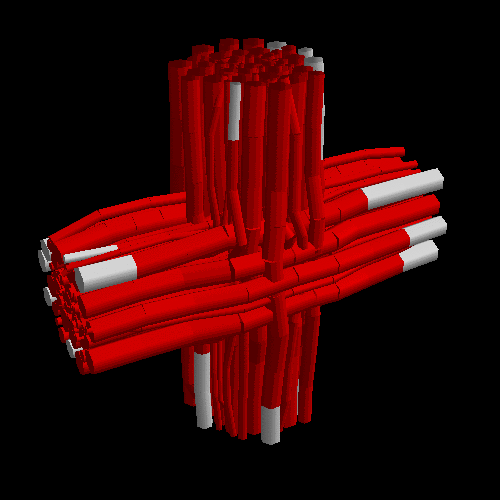
\includegraphics[width=\tikzwidth]{gfx/fastpli/solver-10}&&
    \includegraphics[width=\tikzwidth]{gfx/fastpli/solver-20}&&
    \includegraphics[width=\tikzwidth]{gfx/fastpli/solver-50}&&
    \includegraphics[width=\tikzwidth]{gfx/fastpli/solver-99}\\
    \multicolumn{7}{X}{
    \vspace{-1ex}
    \tikzset{external/export=false} \tikz \draw[->,black](0,0)--++(1,0) node[below, midway] {$\mathit{time}$};}
    \vspace{-1ex}
    \end{tabularx}
    % {\raggedright \tikzset{external/export=false} \tikz \draw[->,black](0,0)--++(1,0);}
	\caption{Exemplary visualization in the collision solving process. The red color indicates that a collision is detected in the fiber segment.}
	\label{fig:vis_solver}
\end{figure}
% 
This allows the user to get direct feedback, \eg{} after each step, to adjust the initial fiber configuration or boundary conditions.
It is written in \cpp{} and \ac{OpenGL} \textit{v2} \cite{isocpp, khronos}.
This implementation uses \code{gluCylinder} to represent a nerve fiber segment.
This is not the fastest approach, but it is still fast enough compared to the computation time of a single step in the collision algorithm.
\par
% 
A further advanced interactive tool is also available as open source, the FAConstructor, which was developed by Jan Reuter as part of his bachelor thesis \cite{Reuter2019}.
It provides additional interactive methods for creating nerve fiber models and was written in \textit{OpenGL\,v3}.
% 
% 
% 
\subsection{Transparent objects and cells}
%
In \cref{sec:medusa} the need of transparent objects is necessary.
Not only the outer hull of the myelin, but also the inner axon needs to be seen in the visualization.
Additionally, cells, \eg{} astrocytes, have to be visualized.
For this purpose, the former algorithm was rewritten.
For the transparent effects the algorithm needs to know the order in which the objects or triangular surfaces needs to be rendered.
This means, that the triangular surfaces have to be sorted in z-direction, \ie{}, the view direction.
To order the triangular surfaces, they first have to be calculated.
The fiber segments are no longer represented as a cylinder, but as \ac{CC} which consist out of a hexagonal grid (see \cref{fig:vis_mesh}).
\par
%
\begin{figure}[!t]
    \centering
    \setlength{\tikzwidth}{0.75\textwidth}
    \inputtikz{gfx/model/vis_a}
	\caption{Generate a mesh for visualization. A mesh perpendicular to the fiber trajectory is calculated from n points. Triangles defined by these points are used as surfaces for the visualization of the object. Normal vectors can be used to smooth the visualization, and flash effects contribute to a more natural representation.}
	\label{fig:vis_mesh}
\end{figure}
% 
This is a huge amount of computational resources.
It is not yet included in the \ac{fastPLI} package.
The resulting visualization is shown in \cref{fig:medusa_8b}.
% 
% 
% 
\section{Medusa - sphered nerve and cell modelling}
\label{sec:medusa}
%
The algorithm described above for generating dense \ac{WM} fiber models can also be applied in \ac{dMRI}.
% 
In \ac{dMRI} the movement and interaction of water molecules with the fiber models is simulated.
When the water molecules collide with the surface of a fiber segment, the molecules behavior, like diffusion though the surface, must be taken into account.
This applies not only to nerve fibers but also to other cell types.
Since the \ac{WM} consists not only of axons, but also of other cells such as glial cells, astrocytes and olegodendrites, these are also changing the signal of the \ac{dMRI}.
\par
% 
Therefore, an additional algorithm was developed in collaboration with Kevin Ginsburger and Cyril Poupon (Neurospin, \ac{CEA}).
This algorithm called \ac{MEDUSA} \cite{Ginsburger2019} works similarly to the algorithm described above, but models the 3D objects as spheres rather than pipe segments.
This has the advantage that the objects are simpler, which leads faster collision checking calculations.
Additionally, the spheres are also used to represent other type of cells.
The overall volume of a cell is represented the sum of all spheres corresponding to the cell (see \cref{fig:medusaCell}).
In this way any shape is possible.
To generate realistic shaped cells this algorithm is specialized to produce olegodendrites and Astrocytes.
\par
% 
Another focus of the algorithm is to be able to generate a volume from statistical parameters such as density and angular dispersion \cite[Ginsburger2019, ginsburgerDis2019].
Analogous to the \cref{sec:Solver} algorithm, the collisions of the objects are checked and slowly pushed apart until no more collisions can be detected.
The usage of the statistical parameters allows generating a general purpose library of volumes filled with nerve fibers and cells (see \cref{fig:medusa_8a}).
\par
% 
The disadvantage of the spheres is that for the representation of tubular objects many more spheres and thus objects for collision control are needed.
Therefore, the algorithm was implemented on the \ac{GPU} with an axis aligned bounding box search algorithm \cite{Karras2012}.
% 
% 
%
\subsection{Algorithm}
%
Since all objects are represented as a collection of spheres (see \cref{fig:medusaCell})
\begin{align}
    \mathcal{S} = \{ (x_i,y_i,z_i,r_i) : i \in \{0, 1, ..., n_\text{objects}-1\}  \}
\end{align}
%
\begin{figure}[!t]
    \centering
    \setlength{\tikzwidth}{0.75\textwidth}
    \subcaptionbox{modified from \cite{Ginsburger2019}. Outer blue spheres myelin, inner red spheres axon}
    [0.75\textwidth]{\inputtikz{gfx/model/medusa/medusa_spheres}}
    \\[2em]
    % 
    \subcaptionbox{Cell aproximation by overlapping spheres.}
    [0.75\textwidth]{\inputtikz{gfx/model/medusa/medusa_cells}}
    \caption{\ac{MEDUSA} sphere approximation.}
    \label{fig:medusaCell}
\end{figure}
%
, a collision occurs when
%
\begin{align}
d<r_i+r_j \enspace \text{with} \enspace d = \abs{\vec{p}_i - \vec{p}_j}
\end{align}
%
However, since adjacent spheres in a fiber collide when the fiber is densely populated, they must be excluded if the length of the partial trajectory is smaller than the sum of the radii of the two spheres:
\begin{align}
\text{ignore if} \enspace \sum_{n=i}^{j-1} \, \abs{\vec{p}_n - \vec{p}_{n+1}} \leq  r_i + r_j 
\end{align}
%
Spheres inside cell bodies are not checked for collisions because their volume is approximately equal to the volume of the cell.
\par
%
The calculation of the collisions is performed using the GPU architecture.
For this first implementation, the algorithm \name{AxisAligedSortedSearch} \cite{Karras2012} is used.
It sorts the spheres along an axis, \obda{} x-axis, and for each sphere $i$ searches for the first and last possible collision on that axis.
This results in a list of spheres $\mathcal{C}_i$ to be tested:
\begin{align}
\begin{split}
\mathcal{C}_i = \{ s \in \mathcal{S} \mid \abs{s_i.x - s_j.x} < r_i+r_j \}
\end{split}
\end{align}
%
The algorithm (see \cref{alg:medusa_collision}) described above is currently used for volumes of about $\SI{200}{\micro\meter}$ for different number of fiber populations and other properties (see \cref{fig:medusa_8a}).
%
\begin{lstfloat}[!t]
	\lstinputlisting[style=cpp]{code/medusa.cu}
	\caption{Pseudocode of \acs{MEDUSA}s collision checking.}
	\label{alg:medusa_collision}
\end{lstfloat}
% 
For this volume size, the algorithm is fast enough for current use.
However, there are more advanced algorithms that can be used here.
One promising technique is the use of a \name{Bounding Box Hierarchy} \cite{Karras2012}.
%
\begin{figure}[!t]
    \centering
    \subcaptionbox{Cubic volumes with different number of fiber populations and volume fractions (VF) are generated.}
    [0.75\textwidth]{\label{fig:medusa_8a}
    \resizebox{0.75\textwidth}{!}{
    \includegraphics{gfx/model/medusa/8.jpg}}}
    \\[2em]
    \subcaptionbox{Exemplary visualization of a volume filled with a single fiber population and astrocytes.}
    [0.75\textwidth]{\label{fig:medusa_8b}
    \resizebox{0.75\textwidth}{!}{
    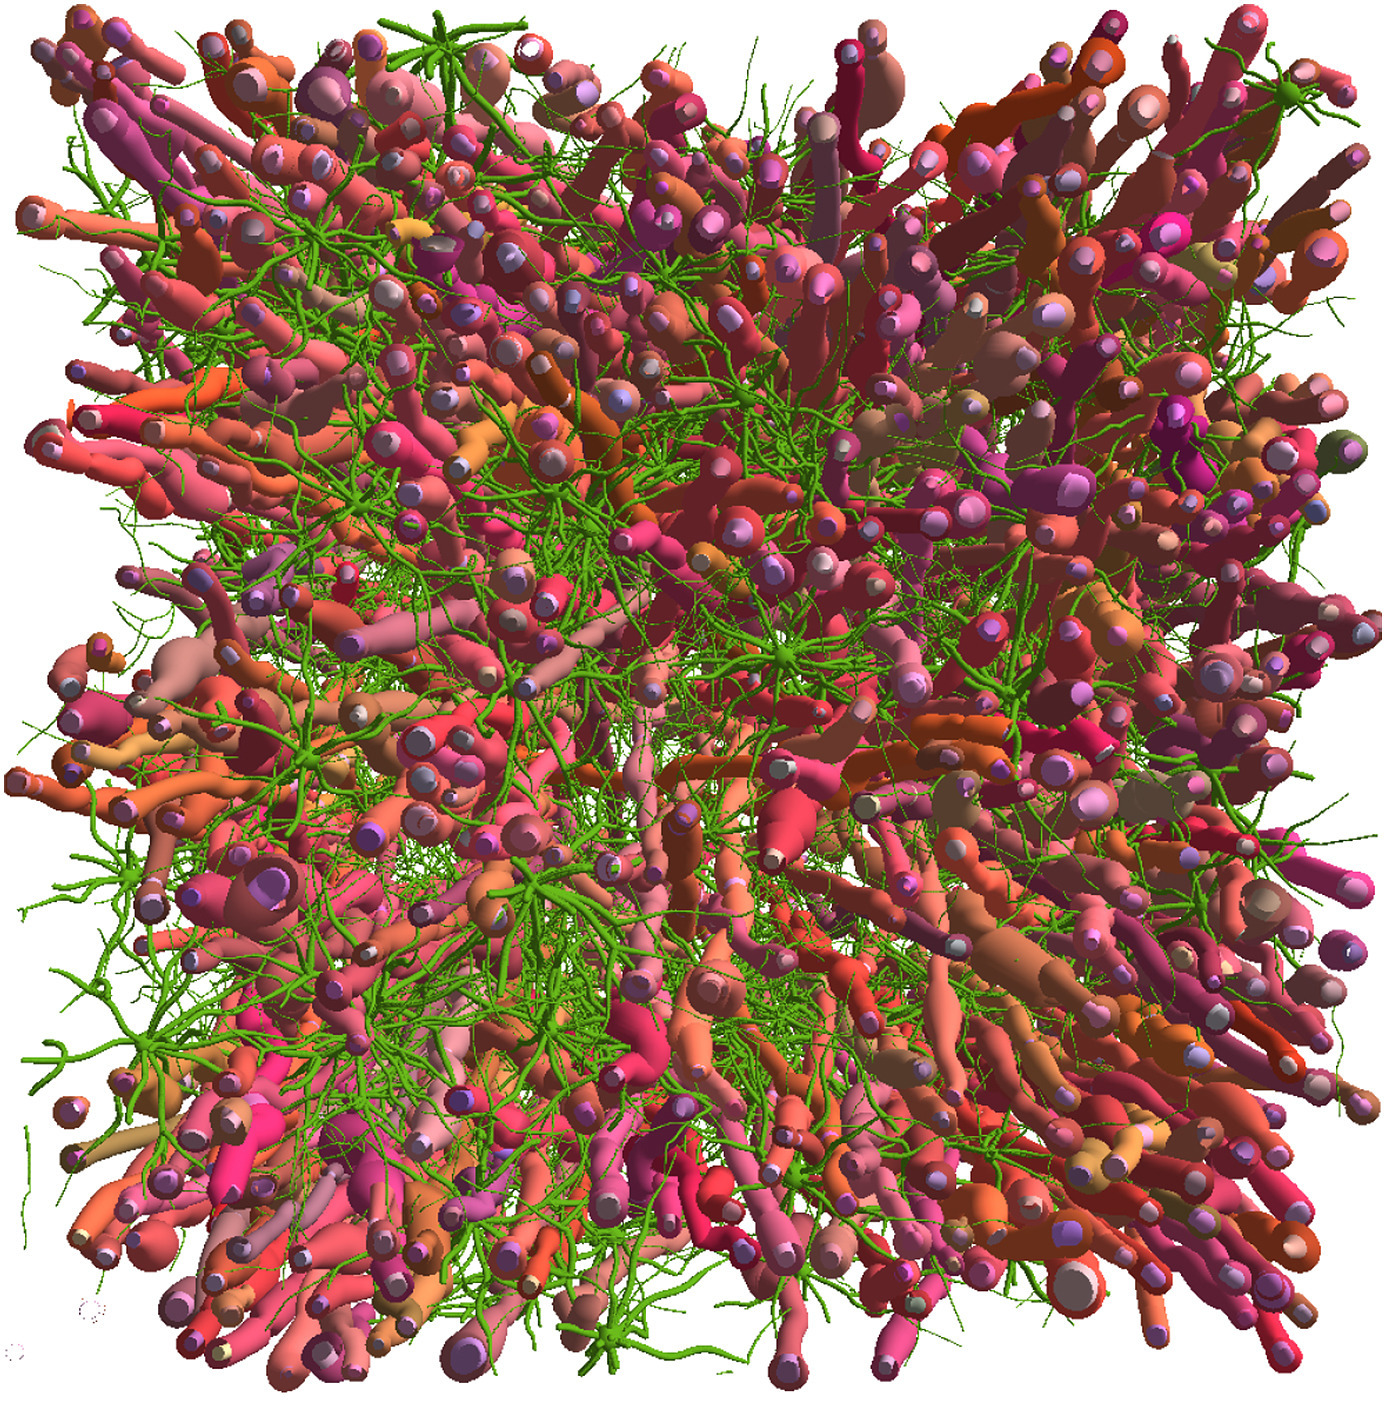
\includegraphics{gfx/model/medusa/11_.jpg}}}
	\caption{Original images from \cite{Ginsburger2019}.}
	\label{fig:medusa_8}
\end{figure}